\documentclass[twoside,UTF8]{EPURapport}
%\usepackage{listings}

%\renewcommand{\lstlistlistingname}{Liste des codes}
%\renewcommand{\lstlistingname}{Code}

%\addextratables{%
%	\lstlistoflistings
%}

%\swapAuthorsAndSupervisors
\nolistoffigures
\nolistoftables


\usepackage{amsmath}
\usepackage{amsfonts}
\usepackage{amssymb}

\usepackage{float}
%\usepackage{color}
\usepackage{array}
\usepackage{multirow}
%\usepackage{xcolor}
\usepackage{supertabular}
\usepackage{longtable}
\usepackage{algorithmic}
\usepackage{algorithm}
\usepackage{hyperref}

\usepackage{graphicx}
\usepackage{caption}
\usepackage{subcaption}


\renewcommand{\algorithmicrequire}{\textbf{Entrées et pr\'{e}condition:}}
\renewcommand{\algorithmicensure}{\textbf{Sorties et postcondition:}}
\renewcommand{\algorithmicend}{\textbf{fin}}
\renewcommand{\algorithmicif}{\textbf{si}}
\renewcommand{\algorithmicthen}{\textbf{alors}}
\renewcommand{\algorithmicelse}{\textbf{sinon}}
\renewcommand{\algorithmicelsif}{\algorithmicelse\ \algorithmicif} 
\renewcommand{\algorithmicendif}{\algorithmicend\ \algorithmicif} 
\renewcommand{\algorithmicfor}{\textbf{pour}}
\renewcommand{\algorithmicforall}{\textbf{pour tout}} 
\renewcommand{\algorithmicdo}{\textbf{faire}}
\renewcommand{\algorithmicendfor}{\algorithmicend\ \algorithmicfor} 
\renewcommand{\algorithmicwhile}{\textbf{tant que}}
\renewcommand{\algorithmicendwhile}{\algorithmicend\ \algorithmicwhile} 
\renewcommand{\algorithmicloop}{\textbf{boucle}}
\renewcommand{\algorithmicendloop}{\algorithmicend\ \algorithmicloop} 
\renewcommand{\algorithmicrepeat}{\textbf{répéter}}
\renewcommand{\algorithmicuntil}{\textbf{jusqu'à}}
\renewcommand{\algorithmictrue}{\textbf{vrai}}
\renewcommand{\algorithmicfalse}{\textbf{faux}}
\renewcommand{\algorithmiccomment}[1]{$/*$~#1~$*/$}
\floatname{algorithm}{Algorithme}
\renewcommand{\listalgorithmname}{Liste des algorithmes}

\thedocument{Décomposition pyramidale du filtre bilatéral}{Développement d’un outil de traitement d’images par filtrage bilatéral}{Décomposition pyramidale du filtre bilatéral}

\grade{Département Informatique\\ 5\ieme{} année\\ 2014 - 2015}

\authors{%
	\category{Étudiants}{%
		\name{Natacha \textsc{Marlio-Ma}} \mail{natacha.marlio-marette@etu.univ-tours.fr}
	}
	\details{DI5 2014 - 2015}
}

\supervisors{%
	\category{Encadrants}{%
		\name{Moncef \textsc{Hidane}} \mail{moncef.hidane@insa-cvl.fr}
	}
	\details{INSA, Blois}
}

\abstracts{}
{}
{}
{}

\begin{document}

\chapter{Décomposition pyramidale}

\paragraph{}
Les différentes méthodes et stratégies misent en place ci-dessous se basent sur l'article \cite{decompo}. 

\paragraph{}
En appliquant le filtre bilatéral sur une image, on peut la décomposer ensuite en une couche de base, c'est à dire l'image résultant du filtre et une couche de détails qui correspond à la différence entre l'image originale et la couche de base. 
\paragraph{}
On notera \textit{g} l'image originale, \textit{u} la couche de base et \textit{v} correspondra à la couche de détails. \textit{BF[$\bullet$]} désigne le filtre bilatéral. 
Soit une décomposition à (\textit{k}+1) niveau, on aura \textit{$u^1$}, ..., \textit{$u^k$} les versions filtrées obtenues de \textit{g}. La dernière version \textit{$u^k$} sera notée \textit{b} et correspondra à la couche de base.
La couche de détail est définie comme suit : 
\begin{equation}
	v^i = u^{i-1} - u^i \textrm{, avec }i=1..k \textrm{ et } u^0=g
\end{equation}

\paragraph{}
L'image original \textit{g} est retrouvé à l'aide de l'équation suivante : 
\begin{equation}
\label{eq:recompo}
	g = b + \sum_{i=1}^{k}v^i
\end{equation}

	\section{Méthodes}

\paragraph{}
La pyramide basée sur le filtre bilatéral peut être construite de deux façons différentes. Ces deux méthodes sont présentées ci-dessous. Les images sont ensuite reconstruite en utilisant l'équation \ref{eq:recompo}.

\subsection{Méthode n\degre 1}	

\paragraph{}
Cette méthode consiste à itérer le filtre bilatéral sur l'image originale en modifiant uniquement les paramètres $\sigma_s$ et $\sigma_r$. Les séquences \textit{$u^1$}, ..., \textit{$u^k$} sont obtenues en résolvant \textit{k} fois le système suivant : 
\begin{equation}
\label{eq:methode1}
	u^{i+1} = BF[g]
\end{equation}

\subsection{Méthode n\degre 2}		

La deuxième méthode que l'on peut mettre en place consiste à appliquer le filtre bilatéral sur la dernière séquence obtenue, ce qui va donner la formule suivante : 
\begin{equation}
\label{eq:methode2}
	u^{i+1} = BF[u^i]
\end{equation}


	\section{Stratégies}		

\paragraph{}
L'article \cite{decompo} présente deux stratégies à mettre en place afin de réaliser un pyramide basée sur le filtre bilatéral. La première consiste à augmenter $\sigma_s$ et $\sigma_r$ à chaque itération. La seconde stratégie consiste à utiliser la méthode n\degre 2 (équation \ref{eq:methode2}) et faire décroître $\sigma_r$ à chaque itération.

\chapter{Résultats}

\paragraph{}
Les résultats présentés ci-dessous montrent les différentes séquences obtenues ainsi que leur couche de détails et l'image reconstruite. 


\begin{figure}[H]
	\begin{center} 
		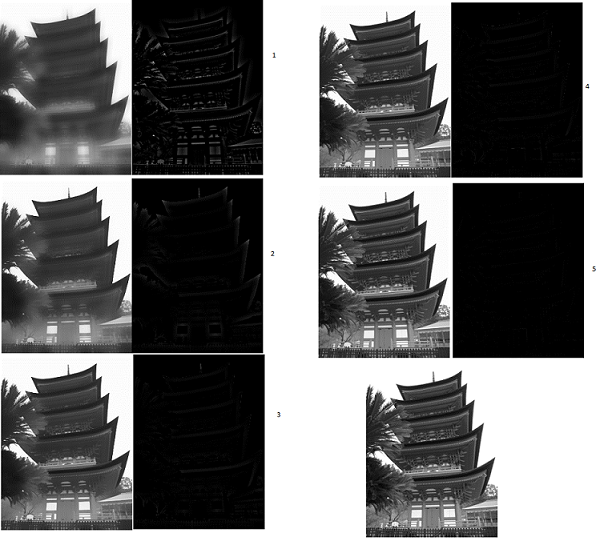
\includegraphics[]{images/pyramide1_rdiv2__36_100_IM088.png} 
	\end{center} 
	\caption{Décomposition pyramidale (méthode 1 et stratégie 2 - $\sigma_r$ divisé par 2), paramètre de départ $\sigma_s$=36 et $\sigma_r$=100}
\end{figure} 

\begin{figure}[H]
	\begin{center} 
		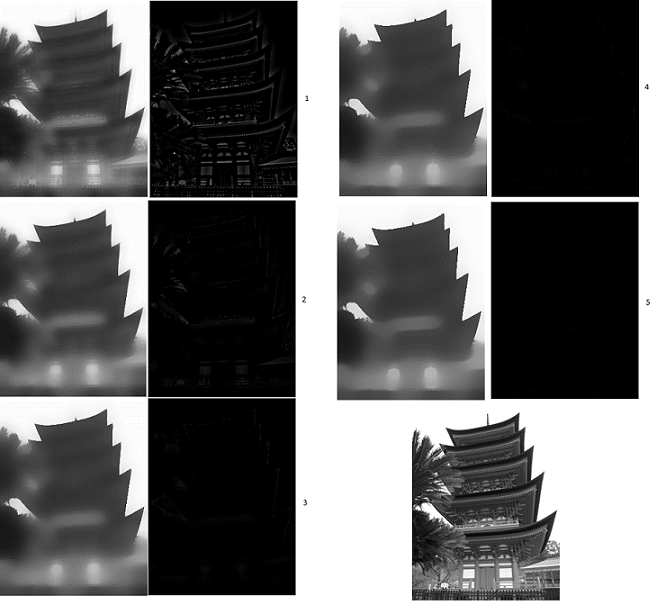
\includegraphics[]{images/pyramide2_rdiv2__36_100_IM088.png} 
	\end{center} 
	\caption{Décomposition pyramidale (méthode 2 et stratégie 2 - $\sigma_r$ divisé par 2), paramètre de départ $\sigma_s$=36 et $\sigma_r$=100}
\end{figure}

\begin{figure}[H]
	\begin{center} 
		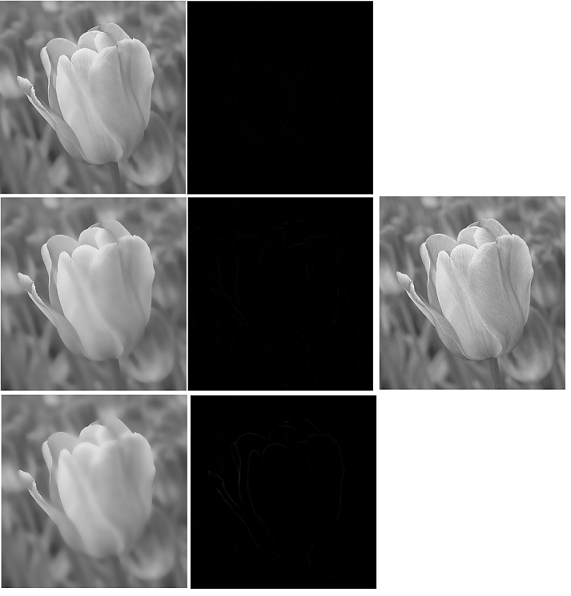
\includegraphics[]{images/pyramide1_x2__4_10_flower.png} 
	\end{center} 
	\caption{Décomposition pyramidale (méthode 1 et stratégie 1 - facteur 2), paramètre de départ $\sigma_s$=4 et $\sigma_r$=10}
\end{figure}



\bibliography{biblio}
\bibliographystyle{unsrt}
\addcontentsline{toc}{chapter}{Bibliographie}

\end{document}